% fig04_ioffe_profile.tex — Ioffe-Pritchard mirror-pair on-axis |B(z)| profile.
% Compiled by the paper Makefile via `make figures` (pdflatex on the snippet).
%
% Data: §Inheritance + companion/verify-ledger.json (ioffe_* atoms).
% Two coaxial loops a=0.10 m, I=1e5 A, separation s=0.40 m (coils at z=+-0.20 m).
% On-axis superposition B(z) = B_loop(z-s/2) + B_loop(z+s/2),
%   B_loop(zeta) = mu0*I*a^2 / (2*(a^2+zeta^2)^{3/2}).
% s/a = 4 > 1  =>  z=0 is a genuine on-axis MINIMUM (magnetic bottle).
% Reference anchors (verify atoms): B_min(0)=0.1124 T, B_coil(+-0.20)=0.6373 T.
% The curve below uses the exact closed form; the marked points are the
% registered verify atoms (the well bottom and the coil-plane maxima).
%
% Manual single-shot compile (debug):
%   pdflatex -interaction=nonstopmode -halt-on-error fig04_ioffe_profile.tex
\documentclass[border=4pt]{standalone}
\usepackage{tikz}
\usepackage{pgfplots}
\pgfplotsset{compat=1.18}
\begin{document}
% mu0*I*a^2/2 = (1.25663706212e-6 * 1e5 * 0.01)/2 = 6.2831853106e-4
% B_loop(zeta) = 6.2831853106e-4 / (0.01 + zeta^2)^1.5
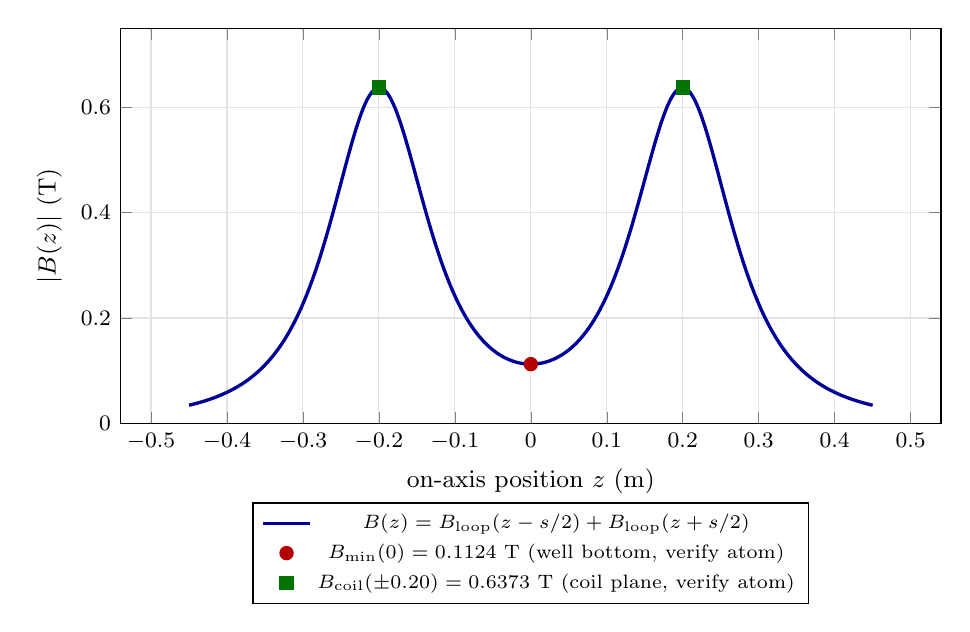
\begin{tikzpicture}
\begin{axis}[
  width=12cm, height=6.6cm,
  domain=-0.45:0.45, samples=181,
  xlabel={on-axis position $z$ (m)},
  ylabel={$|B(z)|$ (T)},
  tick label style={font=\footnotesize},
  label style={font=\small},
  ymin=0, ymax=0.75,
  ymajorgrids, xmajorgrids, grid style={gray!22},
  legend style={font=\scriptsize, at={(0.5,-0.20)}, anchor=north, legend columns=1},
]
% mirror-pair superposition, coils at z = +- 0.20 m
\addplot[blue!60!black, very thick, smooth] {
  6.2831853106e-4/((0.01+(x-0.20)^2)^1.5)
  + 6.2831853106e-4/((0.01+(x+0.20)^2)^1.5)
};
\addlegendentry{$B(z)=B_{\mathrm{loop}}(z-s/2)+B_{\mathrm{loop}}(z+s/2)$}
% marked verify atoms
\addplot[only marks, mark=*, mark size=2.4pt, red!70!black] coordinates {(0,0.1124)};
\addlegendentry{$B_{\min}(0)=0.1124$ T  (well bottom, verify atom)}
\addplot[only marks, mark=square*, mark size=2.4pt, green!45!black] coordinates {(-0.20,0.6373) (0.20,0.6373)};
\addlegendentry{$B_{\mathrm{coil}}(\pm0.20)=0.6373$ T  (coil plane, verify atom)}
\end{axis}
\end{tikzpicture}
\end{document}
